\section{Implementation and Evaluation Methodologies}

The experiments realized in this study were written in the Python programming language (version 3.8.8)~\cite{python}, using the following libraries:

\begin{itemize}
  \item Python Standard Library 3.8.8, for the data types, functional programming, file and directory access, data compression, text processing~\cite{python_standard_library}
  \item Matplotlib, for the plot generations (v3.3.4)~\cite{matplotlib}
  \item Numpy, for scientific computations (v1.20.2)~\cite{numpy}
  \item SciPy, for scientific computations (v1.4.1)~\cite{scipy}
  \item Scikit-learn, for machine learning algorithms implementations (v0.24.1)~\cite{sklearn}
  \item BCubed, to compute the BCubed family metrics (v1.5)~\cite{bcubed_gh}
  \item AdjustText, for automatics text adjustments in plots (v0.7.3)~\cite{adjustText}
  \item Tqdm, to have progress bars for heavy computations (v4.60.0)~\cite{tqdm}
\end{itemize}

The methods proposed are written in Python files (standard text files, extension .py).
Instead, the experiments are contained in a special file format called IPython Notebook (extension .ipynb)~\cite{jupyter}.
A Jupyter environment is required to run these files.
For instance, the JupyterLab environment allows markdown annotation, the possibility to run only portions of codes and even new code in the same Python kernel.
By running each code portion in the same Python kernel, this allows to keep in RAM heavy computations results.
This allows the programmer to dynamically implement and optimize the methods.

The complete source code can be found on GitHub~\footnote{\url{https://github.com/TheRaphael0000/master_thesis}} (see Figure~\ref{fig:qr_code_repository}).

\begin{figure}
  \centering
  \caption[Source code repository, QR Code]{Source code repository QR Code}
  \label{fig:qr_code_repository}
  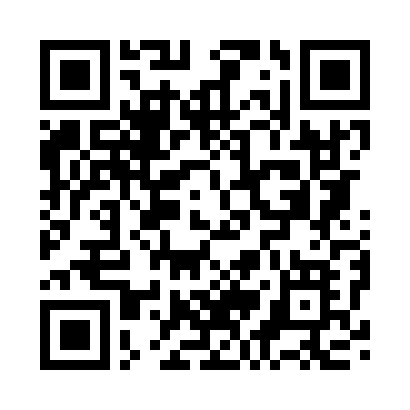
\includegraphics[width=0.8\linewidth]{img/qr_code_repository.png}
\end{figure}
